\chapter{Stand der Technik}
\label{chap.tech}
\prever{
%\red[TODO:\\
%Lokalisation mobiler Systeme in Gebäuden etc.\\
%Augmented Reality inkl. Interaktion mit Projektionen\\
%Handgeführte Lokalisationssysteme (Ohne Projektion)\\
%Bilder von Systemen?\\
%Lokalisation bisschen näher beschreiben/kurze Einführung -> Lokalisation ist Grundvoraussetzung für Betrieb des aufgebauten Systems\\
%Umgebung und Transformation erklären\\
%Wann und wie Karte definieren?\\
%Distanzsensoren oder Entfernungsmesser?\\
%Quelle warum Definition von Deskriptoren häufig nicht generalisierbar\\
%AR-Paper etwas näher ausführen -> 2 Sätze\\
%Quelle Jan-Philipp aktualisieren und ausführen\\
%Autorennamen groß oder so? -> textsc\\
%]
%\red[Viele Forschungsgruppen beschäftigen sich mit der Problematik, sowohl Lokalisation in bekannter als auch unbekannter Umgebung.
%Da das Ziel des entwickelten Systems in der Lokalisation in bekannter Umgebung liegt wird sich bei der Darstellung der bisherigen Forschungsansätze auf diesen Bereich konzentriert. Da das entwickelte System aufgrund seiner Komponenten dafür ausgelegt ist, die Lokalisation auf Basis von Tiefen- und Farbinformationen durchzuführen werden an dieser Stelle Ansätze, welche auf anderen Verfahren wie Ortung von Funkwellen basieren, ebenfalls nicht näher ausgeführt.]\\
}

Da sich die geplante Anwendung des \kps{s} in verschiedene Funktionsbereiche gliedern lässt, soll im Folgenden ein Überblick über den aktuellen Stand der Technik innerhalb der jeweiligen Bereiche gegeben werden. Darüber hinaus werden Systeme vorgestellt, welche eine mit dem in dieser Arbeit entwickelten \kps{} vergleichbare Funktionalität in einem oder mehreren Bereichen bieten.

\section{Lokalisationsverfahren}
\label{chap:mcl}
Die Lokalisation mobiler Systeme in bekannten Umgebungen ist Gegenstand aktueller Forschungsvorhaben. Das Ziel liegt darin, die Pose\footnote{Die Pose eine Systems umfasst die Beschreibung seiner Position und Orientierung bezogen auf die räumlichen Freiheitsgrade.} des Systems innerhalb der realen Umgebung zu bestimmen. Durch vorhergehende Abbildung der betrachteten Umgebung in Form einer Datenstruktur (Karte), können über einen Abgleich mit aufgenommenen Sensordaten die Koordinatentransformationen zwischen dem mobilen System und der realen Umgebung bestimmt werden. Die Ermittlung der Systempose stellt eine Grundvoraussetzung für den Betrieb des aufgebauten \kps{s} dar. Im Hinblick auf den betrachteten Anwendungsfall beschränkt sich der folgende Überblick auf die Lokalisation mobiler Systeme in Innenräumen. Da die Lokalisation des Systems ohne externe Sensorik erfolgen soll, werden darüber hinaus nur Verfahren und Algorithmen betrachtet, welche die Pose des Systems auf Basis der eigenen Sensordaten bestimmen.\\

Besonders in der Robotik hat sich die Selbstlokalisation mobiler Systeme in den letzten Jahrzehnten zu einem wichtigen Forschungsbereich entwickelt, da sie eine Voraussetzung für die autonome Navigation von Robotersystemen darstellt. Die Anwendungsbereiche werden dabei nach Verfahren zur globalen und lokalen Lokalisation unterschieden. Bei der globalen Lokalisation soll die absolute Pose des Systems innerhalb seiner Umgebung ermittelt werden. Als lokale Lokalisation wird hingegen die Bestimmung einer relativen Transformation zwischen dem vorhergehenden und dem aktuellen Zustand bezeichnet. Während die globale Lokalisation damit meist angewendet wird, um die initiale Pose in einer bekannten Umgebung festzulegen, dient die lokale Lokalisation dazu, die Veränderungen der Systempose kontinuierlich zu verfolgen (Tracking). Die zur gleichen Zeit betrachtete Anzahl möglicher Posen des Systems (Hypothesen) führt zu einer weiteren Kategorisierung innerhalb der Verfahren. Während unimodale Lokalisationsverfahren sich auf eine Hypothese zur Bestimmung der Systempose beschränken, werden bei multimodalen Lokalisationsverfahren verschiedene Hypothesen parallel betrachtet \cite{Hertzberg2012}.
%Im Folgenden soll ein Überblick über verbreitete Lokalisationsansätze gegeben werden.
%Unimodale Ansätze berücksichtigen jeweils nur eine Pose, während bei multimodalen Verfahren mehrere Posen gleichzeitig aufrechterhalten werden.
\subsection{Unimodale Lokalisationsverfahren}
\label{chap.unimod}
Da bei unimodalen Verfahren nur eine mögliche Pose des Systems betrachtet wird, erfordert der Einsatz im Rahmen einer globalen Lokalisation meist eine  plausible Hypothese des Anfangszustands. In diesem Fall kann angenommen werden, dass die betrachtete Pose bereits eine hinreichende Annäherung an die wahre Systempose darstellt. Vornehmliche Anwendung finden unimodale Lokalisationsverfahren daher im Bereich der lokalen Lokalisation.\\

Einen grundlegenden Ansatz stellt das sogenannte \textit{Scan Matching} dar. Dieses Verfahren bezeichnet den Abgleich (Matching) von Messungen der Umgebung mit vorangegangenen Messungen \cite{Gutmann1996} oder zuvor aufgezeichneten Vergleichsdaten \cite{Gutmann1998}. Durch Bestimmung der maximalen Überlappung kann die translatorische und rotatorische Differenz der Pose bezüglich der Referenz berechnet werden. Als Messwerte werden meist Distanzen betrachtet, welche beispielsweise mit Laser- \cite{Diosi2007} oder Ultraschall-Entfernungssensoren \cite{Burguera2005} aufgezeichnet wurden. Die Berechnung der Transformationsvorschrift zwischen den Zuständen erfolgt auf Basis verschiedener Algorithmen wie dem \textit{Iterative Closest Point} Verfahren \cite{Besl1992}\cite{Lu1994} oder der \textit{Normal Distributions Transformation} \cite{Biber2003}.\\

Das \textit{Line Matching} erweitert diesen Ansatz, indem es die häufig geradlinige Struktur von Innenräumen nutzt. Anstelle einzelner Messpunkte werden Linien aufeinander abgeglichen, wodurch die Robustheit der Lokalisation gesteigert werden kann. Die Linien werden dabei aus den Messwerten extrahiert und mit zuvor erstellten Liniendaten aus der Lokalisationsumgebung verglichen \cite{Cox1991}\cite{Gutmann1999}. Auch ein umgekehrtes Vorgehen ist möglich, in welchem die Liniendaten der Karte in äquidistante Punktmengen transformiert und mit den Daten der Entfernungsmessung abgeglichen werden. In diesem Fall reduziert sich die Berechnung der Überdeckung auf das Abgleichen von Punkten, welches mit den Algorithmen des \textit{Scan Matching} gelöst werden kann \cite{Hertzberg2012}.\\

Eine Erhöhung der Komplexität wird durch die Betrachtung von Polylinien, also zusammenhängenden Linienelementen erreicht \cite{Wolter2004}. Zur Lösung können dabei Algorithmen angewendet werden, welche im Rahmen der computergestützen Bildverarbeitung für das Abgleichen von Formen entwickelt wurden. Weitere Ansätze des \textit{Line Matching} verfolgen die Beschreibung der Liniendaten mittels verschiedener Deskriptoren wie Länge, Abstand und Winkel \cite{Frey2014}\cite{Garulli2005}. Dieses Vorgehen ermöglicht eine kompaktere Darstellung der relevanten Umgebungsmerkmale und bildet den Übergang zu den merkmalsbasierten Lokalisationsverfahren.\\

Die allgemeine Anwendung des Prinzips von Deskriptoren (Features) zur Ermittlung der aktuellen Pose eines Systems beschreibt die merkmalsbasierte Lokalisation (\textit{Feature Matching}). Betrachtet werden je nach Anwendungsfall und verwendeter Sensorik individuelle Merkmale. Neben Distanzmessungen \cite{Tomono2004} werden insbesondere auch Kamerasysteme verwendet, um Features aus der Umgebung zu extrahieren \cite{Se2001}. Kamerasysteme stellen passive Sensoren dar und werden daher weniger von Umgebungsbedingungen beeinflusst als aktive Entfernungssensoren. Die Vielzahl an Informationen, welche sich aus einem Kamerabild extrahieren lassen und die Nähe zur menschlichen Wahrnehmung der Umgebung haben darüber hinaus dazu geführt, dass sich die Verwendung von Bilddaten in der merkmalsbasierten Lokalisation als Basis bewährt hat \cite{Wolf2002}. Auch hier kann somit auf eine Vielzahl von Algorithmen aus der computergestützten Bildverarbeitung zurückgegriffen werden. Die kontinuierliche Bestimmung der Systempose auf Basis visueller Features wird unter dem Begriff der visuellen Odometrie\footnote{Als Odometrie wird in der Robotik die fortlaufende Ableitung der Orientierung und Geschwindigkeit aus Messungen der Raddrehwinkel bezeichnet \cite{Hertzberg2012}.} \cite{Mccarthy2003} zusammengefasst.\\
%Definition der Deskriptoren bei Laserscan etc. schwierig und Anwendungsabhängig -> hauptsächlicher Einsatz von merkmalsbasierter Lokalisation bei visuellen Daten (Kamerabildern) \red[visuelle Odometrie fällt darunter!] SIFT/SURF, PCA.

Ein weiteres unimodales Lokalisationsverfahren stellt die Schätzung und Verfolgung der Systempose mittels eines Kalman-Filters \cite{Kalman1960} dar, welches in \kapitel{chap.kalman} näher beschrieben wird. Dieses Verfahren kann auf den bisher beschriebenen Matching Verfahren aufbauen, ist jedoch nicht auf diese limitiert. Das Kalman-Filter ermöglicht eine Fusion der Sensordaten mit der Odometrie. Ein großer Vorteil dieses Lokalisationsverfahrens liegt somit darin, mehrere Datenquellen in einem Modell vereinen zu können. Die Sensordaten können beispielsweise aus globalen Kartenmerkmalen ermittelt werden \cite{Leonard1991} oder aus der Kombination verschiedener Sensoren \cite{Roumeliotis1997} resultieren. Da das Kalman-Filter die Pose mittels einer Wahrscheinlichkeitsdichtefunktion annähert, eignet es sich besonders unter der Voraussetzung, dass lediglich eine Approximation der initialen Pose vorliegt. Als globales Lokalisationsverfahren bei unbekannter Startpose ist das Kalman-Filter dagegen nur bedingt geeignet. Der Einsatz multimodaler Lokalisationsverfahren ermöglicht es jedoch, diese Limitierung durch parallele Verwendung multipler Kalman-Filter zu überwinden.
%Anwendung des Kalman-Filters auf mehrere Hypothesen führt zu multimodalen Lokalisationsverfahren. 
%EKF approximiert Verteilung lokal als Gaußverteilung

\subsection{Multimodale Lokalisationsverfahren}
Multimodale Lokalisationsverfahren erhalten stets mehrere Hypothesen der Systempose aufrecht. Neben einer globalen Lokalisation ohne Anfangshypothese ermöglichen sie dadurch auch das Wiedererlangen korrekter Posen nach fehlgeschlagener Lokalisation. Im Falle einer fehlerhaften Lokalisation ist beispielsweise das \textit{Scan Matching} zwar in der Lage die Überdeckung zwischen Sensordaten und lokaler Kartenumgebung zu optimieren, der Algorithmus erkennt jedoch nicht, ob es sich dabei auch um ein globales Optimum handelt. Wichtig wird dieser Aspekt insbesondere beim \textit{kidnapped robot scenario}, bei welchem das System im Betrieb aus seiner bekannten Pose in eine unbekannten Pose gebracht wird, ohne dabei Sensordaten auszuwerten \cite{Yic2011}. Multimodale Verfahren können dieser Situation begegnen, indem sie stets eine gewisse Anzahl an Posen betrachten und in jedem Lokalisations-Schritt zufällige Posen in die Betrachtung integrieren.\\

Das bei der \textit{Markov-Lokalisation} angewendete Prinzip basiert auf einer Diskretisierung des Posenraums. Für jeden Freiheitsgrad des Systems wird eine Rasterkarte erstellt, in welcher die Gitterzellen mögliche Posen innerhalb des diskreten Raumes repräsentieren. Jede Hypothese wird über eine Wahrscheinlichkeitsdichte abgebildet, welche beispielsweise auf Basis des Kalman-Filters bestimmt wird \cite{Hertzberg2012}. Initialisiert wird die \textit{Markov-Lokalisation} entweder als eine Gleichverteilung über alle Zellen oder als Normalverteilung um definierte Startposen \cite{Hertzberg2012}. In jedem Schritt der Lokalisation werden anschließend Odometrie- und Sensordaten verarbeitet, um die Wahrscheinlichkeitsdichte der Gitterzellen anzupassen. Da selbst bei deutlichem Anstieg der Probabilität einer Pose auch die weiteren Posen in der Betrachtung erhalten bleiben, ist das Verfahren stets in der Lage auf eine fehlerhafte Lokalisation zu reagieren.\\

%Die globale Lokalisation erfolgt bei der \textit{Markov-Lokalisation} entweder durch Initialisierung mit einer Gleichverteilung über alle Zellen, oder durch eine Initialisierung mit Normalverteilung und geringer Varianz um die Hypothesen der Startpositionen \cite{Hertzberg2012}.\\

Die Diskretisierung und gleichzeitige Betrachtung aller möglichen Posen ist mit großem Rechenaufwand verbunden. Der Ansatz der \textit{Monte-Carlo-Lokalisation} verringert den benötigten Aufwand, indem eine ausgewählte Stichprobe betrachtet wird. Die Elemente der Stichprobe entsprechen möglichen Posen und werden als Partikel bezeichnet. Neben dem diskreten Posenraum können die Partikel auch aus dem kontinuierlichen Posenraum gewählt werden, wie er häufig bei mobilen Systemen vorliegt \cite{Fox2001}. Die Kontrolle über die Partikelanzahl ermöglicht es zudem, den Algorithmus auf die verfügbaren Rechenressourcen abzustimmen \cite{Thrun2001}. Darüber hinaus kann eine Vielzahl verschiedener Wahrscheinlichkeitsverteilungen als Basis des Verfahrens verwendet werden. Die \textit{Monte-Carlo-Lokalisation} ist dadurch in der Lage, die globale und lokale Lokalisation mit hoher Genauigkeit zu realisieren \cite{Thrun2005}. Zusammen mit der hohen Effizienz des Ansatzes führt dies dazu, dass er bei der Lokalisation mobiler Systeme der \textit{Markov-Lokalisation} überlegen ist \cite{Fox2001}.

%\red[Monte Carlo etc. ->Buch\\]
%\red[smartphone lokalisierung thematisieren aber verwendet externe Sensorik zur Positionsbestimmung]

%\red[In der Robotik wird die fortlaufende Ableitung der Orientierung und Geschwindigkeit aus Messungen der Raddrehwinkel als Odometrie bezeichnet. \cite{Hertzberg2012}\\]

\prever{
%\red[Wie Quelle \cite{Hertzberg2012} für gesamten Lokalisationsabsatz referenzieren?]
}
%\red[Welche Lokalisationsverfahren gibt es. Allgemein und speziell für handgeführte Systeme.]\\

\prever{
%\section{\red[3D-Kameras in der Lokalisation]}
}
\section{Lokalisation auf Basis von 3D-Kameras}
Die beschriebenen Verfahren und Algorithmen haben sich besonders bei der Lokalisation in zweidimensionalen Umgebungen bewährt, obwohl sie meist unabhängig von der Anzahl an Dimensionen formuliert sind. Die zunehmende Verbreitung von zugleich kostengünstigen und leistungsfähigen 3D-Kameras führt jedoch dazu, dass der Anwendungsbereich vermehrt auch auf dreidimensionale Umgebungen erweitert wird. Die dreidimensionale Lokalisation ist insbesondere dann von Bedeutung, wenn das System sich in mehr als einer Ebene bewegen kann. Während die Pose des Systems in zweidimensionalen Umgebungen durch zwei translatorische und einen rotatorischen Freiheitsgrad beschrieben werden kann, verdoppelt sich die Anzahl an Freiheitsgraden durch die zusätzlich betrachtete Dimension. Die Beschreibung der Systempose erfolgt nun über drei translatorische und drei rotatorische Freiheitsgrade.\\

Die Lokalisation in dreidimensionalen Umgebungen erfordert geeignete dreidimensionale Karten. Liegen keine Modelldaten vor, können sie auf Basis von Sensordaten aus der realen Umgebung rekonstruiert werden. 3D-Kameras werden dabei in Verfahren eingesetzt, welche die Lokalisation während der Rekonstruktion der Umgebung durchführen \cite{Durrant2006}. Bewegungen mobiler Systeme im dreidimensionalen Raum führen darüber hinaus häufig dazu, dass keine Odometriedaten mehr ermittelt werden können. Dies ist insbesondere bei fliegenden \cite{Huang2011} und hand- oder körpergeführten Systemen \cite{Fallon2012} der Fall. Die Auswertung von Tiefen- und Farbinformationen ermöglicht es jedoch, dies durch die zuvor beschriebene visuelle Odometrie zu kompensieren \cite{Whelan2013robust}. Insgesamt sind 3D-Kameras damit gut als Sensoren für Lokalisationsverfahren in dreidimensionalen Umgebungen geeignet \cite{Cunha2011} \cite{Eriksson2012}. Dabei sollten sie jedoch weniger als Ersatz, sondern vielmehr als anwendungsabhängige Alternative zu Sensoren wie Laser-Entfernungssensoren betrachtet werden, da der Messbereich von 3D-Kameras bezüglich Distanz und Sichtfeld meist deutlich von anderen Entfernungssensoren abweicht.
%\red[Featurebasierte Lokalisation (RGB-D SLAM, Fovis)\\
%Markerbasierte Lokalisation]\\

\section{Projektorbasierte Augmented Reality}
Die Überlagerung oder Vereinigung von virtueller und realer Umgebung wird als \textit{Augmented Reality} (AR) bezeichnet \cite{Azuma1997}. Eine dreidimensionale Registrierung setzt reale und virtuelle Objekte bezüglich ihrer Pose in Beziehung und ermöglicht die Interaktion zwischen den Objekten der beiden Welten. Die Umgebung des menschlichen Beobachters wird somit um virtuelle Elemente ergänzt. Neben normalen oder transparenten Bildschirmen werden dabei insbesondere Projektoren zur Visualisierung der virtuellen Daten eingesetzt.\\

\nomenclature[a]{AR}{Augmented Reality}

Anwendungsmöglichkeiten für AR finden sich dabei in verschiedensten Gebieten. In der Medizin können Ärzte durch Visualisierung von Gefäßstrukturen und Informationen zur Operationsplanung in der Chirurgie unterstützt werden \cite{Nicolau2011}. Auch die Kommunikationsmöglichkeiten zwischen Arzt und Patient lassen sich durch den Einsatz von AR erweitern, indem anatomische Strukturen direkt auf den Körper des Patienten projiziert werden \cite{Bluteau2005}. Durch visualisierte Zusatzinformationen ermöglicht AR ein interaktives Trainieren von Robotersystemen \cite{DeTommaso2012}. Visuelle Rückmeldungen erlauben dabei iterative Anpassungen des Trainingsvorgangs und ermöglichen die soziale Interaktion für Anwender ohne spezielle Kenntnisse im Bereich der Robotik. Auch in Alltagssituationen lassen sich interaktive Benutzungsschnittstellen realisieren. \textsc{Linder} und \textsc{Maes} haben mit \textit{LuminAR} ein aktuiertes Projektionssystem entwickelt, welches an eine Schreibtischlampe angelehnt ist und die Visualisierung von Informationen und Erkennung von Benutzereingaben ermöglicht \cite{Linder2010}. Virtuelle Modelle lassen sich durch Projektion auf reale Objekte visualisieren, wodurch geometrisch korrekte Abbildungen mit modifizierbaren Erscheinungsformen erzeugt werden \cite{Raskar1999}. Die Kombination mehrerer Projektoren ermöglicht darüber hinaus die Abbildung komplexer Modellumgebungen, beispielsweise von Innenräumen, auf reale Geometrien \cite{Low2001}. Wird zusätzlich auch die Anzahl an Sensoren zur Erfassung der Umgebung erhöht, lässt sich der Interaktionsbereich mit virtuellen Objekten auf multiple, nicht verbundene Oberflächen erweitern \cite{Wilson2010}.\\

%\cite{Gavaghan2012} \red[Handgeführt!]
%\cite{Huber2012} \red[Handy!]
%\red[Erweiterte Definition der AR durch Einblendung von visuellen Informationen\\]

%\red[Low - Life-Sized Projector Based Dioramas -> Hausumgebung auf leere Wände projiziert]\\
%\red[Oh - Projektion von Entertainment/Filmen etc. auf Oberflächen]\\
%\red[Raskar - Table-Top AR, Bringing Physical Models to life]\\
%\red[Huber - Lightbeam -> Interaktion mit Projektionen über Alltagsgegenstände]\\
%\red[Linder - LuminAR -> Interaktion mit Projektion in Büroumgebung]\\
%\red[Wilson - Interaktion zwischen mehreren Oberflächen durch Einsatz mehrerer Projektoren und Kameras]

%\section{Interaktion}
%\red[Benutzerinteraktion basierend auf der Verwendung von Tiefeninformationen. Hauptsächlicher Ansatz ist die Befehlsvorgabe über Gestensteuerung.]\\
%\red[Welche Formen von Benutzerinteraktion gibt es, besonders bezogen auf die Kinect und Projektionssysteme.\\
%(z.B. Omnitouch)]\\

%\red[Wen - Handgesten zur Interaktion in der Chirurgie]\\

\prever{
%\red[\section{Handgeführte Projektionssysteme}]
}
%\subsection{Lokalisation}
%\red[Ein handgeführtes Scanning System, entwickelt von Mair \textit{et al.} \cite{Mair2010}, fusioniert IMU Daten und  \\]

\prever{
%\red[Absätze kombinieren?]
}

%\subsection{Projektion}
Die Miniaturisierung der Projektionstechnologie hat zu einer Entwicklung mobiler und handgeführter Systeme geführt. In den letzten Jahren wurden verschiedene Ansätze untersucht, welche sich mit der Projektion virtueller Zusatzinformationen durch tragbare Systeme befassen. Dabei werden sowohl eigenständige als auch in Smartphones integrierte Projektionssysteme eingesetzt.\\
% Im Folgenden soll ein Überblick über vorhandene handgeführte Projektionssysteme und ihre Anwendungsbereiche gegeben werden.\\

\prever{
%\red[\cite{Kobler2010}]\\
}

In der Chirurgie kann durch tragbare Projektionssysteme die Flexibilität in der Visualisierung während der Operation erhöht werden \cite{Kobler2010} \cite{Gavaghan2012}. Insbesondere die Mobilität des Projektionssystems erhöht dabei im Vergleich zur Verwendung von Monitoren und ortsfesten Projektoren die intuitive Eingliederung in den Operationsprozess, da sich die Darstellung stets auf das Blickfeld des Chirurgen ausrichten lässt. Die Kombination der Projektionssysteme mit chirurgischen Instrumenten ermöglicht eine Verbesserung der Hand-Auge-Koordination während des Eingriffs, indem beispielsweise Navigationshilfen zur Durchführung von Bohrvorgängen direkt auf dem Patienten visualisiert werden \cite{Kobler2012}.\\

Die Navigation innerhalb eines Museums wird von \textsc{Wecker} \textit{et al.} \cite{Wecker2013} mittels handgeführter Projektionssysteme durch die Visualisierung von Karten- und Wegdaten unterstützt. Ein System mit ähnlichem Ziel haben \textsc{Chung} \textit{et al.} \cite{Chung2011} entwickelt. Dieses soll dem Anwender bei der Navigation innerhalb von Gebäuden behilflich sein. Ein Miniprojektor wird dabei in Kombination mit einem Smartphone verwendet, um zusätzliche Informationen bei der Erkennung von Visitenkarten oder Gebäudeplänen zu visualisieren. Die Funktionalität soll dabei an eine Taschenlampe erinnern, welche die Zusatzinformationen sichtbar macht. Auch \textsc{Li} \textit{et al.} \cite{Li2013} stellen ein handgeführtes Projektionssystem vor, welches im Konzept an eine Taschenlampe angelehnt ist. Durch Projektion von Karten- und Wegdaten auf den Boden vor dem Benutzer wird dieser entlang eines Pfades geführt. Im Gegensatz zu \textsc{Chung} \textit{et al.} erfolgt dabei eine kontinuierliche Aktualisierung der Projektion in Abhängigkeit der Position entlang des Weges, welche manuell durch eine Begleitperson erfasst wird. \textsc{Molyneaux} \textit{et al.} \cite{Molyneaux2012} erweitern die Metapher der Taschenlampe und integrieren darüber hinaus eine automatische Lokalisation des handgeführten Projektionssystems. Eine externe Infrastruktur aus 3D-Kameras erkennt und verfolgt die Systempose und ermöglicht dadurch die verzerrungsfreie Projektion beliebiger Zusatzinformationen innerhalb eines Raumes. Durch Infrarot-Kameras am Projektionssystem selbst wird zudem eine Interaktion mit den visualisierten Daten realisiert.\\

Das \textit{SideBySide} Projekt von \textsc{Willis} \textit{et al.} \cite{Willis2011} ermöglicht die Interaktion zwischen Benutzern über handgeführte Projektionssysteme. Jedes System projiziert sowohl ein Bild im sichtbaren Lichtspektrum als auch einen Marker im Infrarot Spektrum. Die Erkennung der Marker durch die Systeme erlaubt das Zusammenspiel der jeweiligen Projektionen der Anwender. Anwendungen findet das System im Austausch von Informationen oder Dateien und in kooperativen Spielen, wie in \abb{fig.projsystems} (a) dargestellt. Einen weiteren Ansatz für kooperative Projektionssysteme liefern \textsc{Robinson} \textit{et al.} \cite{Robinson2012} mit \textit{PicoTales}. Dabei werden handgeführte Projektionssysteme eingesetzt, um gemeinsam animierte Videos zu erstellen. Die Lokalisation erfolgt über das Aufzeichnen von Bewegungsdaten durch eine inertiale Messeinheit. Die Auswertung und Fusion zu einem gemeinsamen Video wird separat nach Abschluss der Interaktion durchgeführt.\\

Das von \textsc{Harrison} \textit{et al.} \cite{Harrison2011} entwickelte \textit{Omnitouch} ist ein körpergeführtes System, welches die Projektion grafischer Benutzungsschnittstellen auf typische im Alltag vorhandene Oberflächen ermöglicht. Das System verfügt neben einem Projektor auch über eine 3D-Kamera zur Detektion von Benutzereingaben. Dadurch wird wie in \abb{fig.projsystems} (b) gezeigt die Funktionalität von Touchscreens abgebildet, so dass typische Anwendungen implementiert werden können, die sonst beispielsweise auf Smartphones oder Tablets genutzt werden. Ein vergleichbarer Aufbau wird von \textsc{Tan} \textit{et al.} \cite{Tan2013} verwendet, um virtuelle Modelldaten auf reale Modelle zu projizieren. Dies ermöglicht die korrekte Darstellung der virtuellen Daten auch bei einem Wechsel der Beobachterperspektive. Die Lokalisation des Systems erfolgt anhand des Abgleichs zwischen Modell und Sensordaten.

\begin{figure}[!ht]
	\begin{center}
	\subfigure[\textit{SideBySide} \cite{Willis2011}]{
		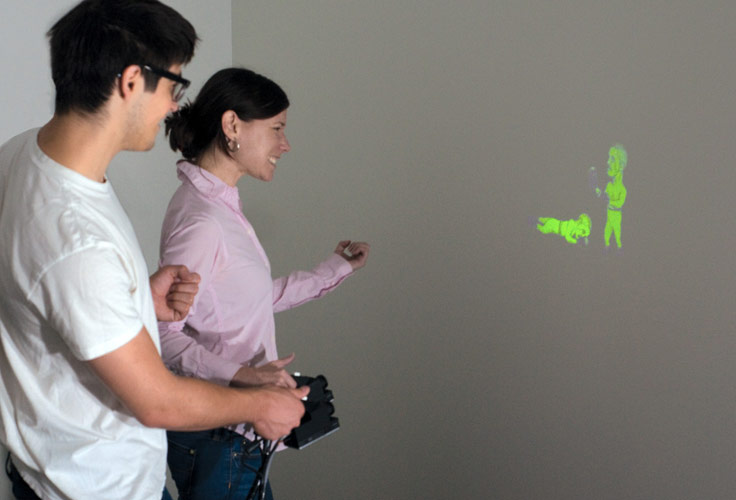
\includegraphics[height=4.8cm]{sidebyside}
	}
	%\hspace{4mm}
	\subfigure[\textit{Omnitouch} \cite{Harrison2011}]{
		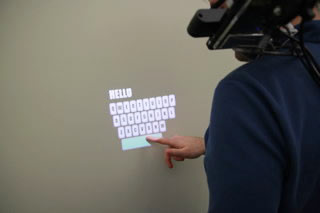
\includegraphics[height=4.8cm]{omnitouch}
	}
	\caption{Beispiele mobiler Projektionssysteme}
	\label{fig.projsystems}
	\end{center}
	%\vspace*{-8mm}
\end{figure}

\prever{
%\red[Abbildungen der Systeme?\\]
}

%Warum der Ansatz?
Wenige der handgeführten Systeme ermitteln ihre Pose innerhalb der Umgebung. Häufig ist lediglich die relative Pose bezüglich definierter Oberflächen oder Objekte Bestandteil der Betrachtung. Systeme, welche eine globale Lokalisation erfordern, verwenden dagegen entweder manuelle oder auf externen Sensoren basierende Lokalisationsverfahren. Die Selbstlokalisation mobiler Systeme ist seit einiger Zeit Forschungsthema und es existiert wie beschrieben eine Vielzahl von Ansätzen, um eine zuverlässige Lokalisation in zwei- und dreidimensionalen Umgebungen zu realisieren. Eine Übertragung auf den Anwendungsbereich handgeführter Projektionssysteme fand bisher jedoch nicht statt.\\

Die vorliegende Arbeit soll die Lücke zwischen der Lokalisation mobiler Systeme und der projektorbasierten AR schließen. Die Anwendungsgebiete werden vereint, indem die Selbstlokalisation eines handführbaren \kps{s} realisiert und darauf aufbauend die interaktive Projektion visueller Zusatzinformationen in der realen Umgebung ermöglicht wird.\\

\prever{
%\red[Zwei Lokalisationsansätze verwendet, globale Lokalisation und visuelle Odometrie]
}

%\red[Verschiedene handgeführte Systeme, welche jedoch entweder auf manueller, externer Lokalisation, oder markerbasierter Lokalisation beruhen. Bei anderen Systemen wird lediglich eine Ausrichtung bzgl der Projektionsoberfläche durchgeführt. Selbstlokalisation ohne Hilfsmittel (externe Sensorik, Marker in Form von KArten o.ä.) bisher nicht behandelt. Lokalisation von mobilen Systemen allerdings seit einiger Zeit Forschungsthema, neuer ist jedoch die 3D Lokalisation. System soll die Brücke bilden zwischen mobilen, autonomen Lokalisationssystemen und handgeführten Projektionssystemen\\]

%\prever{
%\red[OHNE HILFSMITTEL nochmal aufgreifen wenn alternative Lokalisation über Muster o.ä. aufgeführt wird]
%\red[Tan - iSarProjection -> Handgeführtes System, Aufbau sehr ähnlich Kinpro, Lokalisation aber anhand der Modelle auf die dann projiziert wird, eher wie David]\\
%\red[Welche Systeme gibt es zur Projektion von (Modell-)Daten.]\\
%\red[Kobler zitieren]
%}

%\includesvgnew[1]{test}
